%%% Uppsala University presentation beamer template v2.0
%%% provided by Diletta Goglia, IT Department, Uppsala University
%%% email: diletta.goglia@it.uu.se
%%% December, 2023

% This template is the updated version of the "Uppsala University presentation template v1.0" created by Mats Jonsson (mats@mekeriet.se) in March 2021.


\documentclass{beamer}

\usepackage[english]{babel}
\usepackage[utf8x]{inputenc}
\usepackage{hyperref, % clickable links
    graphicx, % include images
    listings, % for code and formatting
    caption, % customization of captions in figures and tables
    stackengine, % custom layouts 
    amsmath, % math env
    xcolor, % extend color support
    multicol, % multiple columns layout
    booktabs, % high quality tables
    lipsum % remove it
}

\usepackage{UU_beamer} % customized style

\def\cmd#1{\texttt{\color{red}\footnotesize $\backslash$#1}}
\def\env#1{\texttt{\color{blue}\footnotesize #1}}

% ------ CODE COLOR DEFINITION ------ %

\definecolor{codered}{rgb}{0.6,0,0}
\definecolor{codeblue}{rgb}{0,0,0.8}
\definecolor{codegreen}{rgb}{0,0.5,0}
\definecolor{almostwhite}{gray}{0.55}
\definecolor{codepurple}{rgb}{0.58,0,0.82}
\definecolor{backcolour}{rgb}{0.95,0.95,0.92}

\lstset{
    basicstyle=\ttfamily\small,
    keywordstyle=\bfseries\color{codeblue},
    emphstyle=\ttfamily\color{codered},   % Custom highlighting style
    stringstyle=\color{codepurple},
    numbers=left,
    numberstyle=\small\color{almostwhite},
    rulesepcolor=\color{red!20!green!20!blue!20},
    frame=shadowbox,
    commentstyle=\color{codegreen},
    captionpos=b    
}

% ------------- PRESENTATION INFO --------------- %
\newcommand{\fullconference}{Memory Technologies - Spring 2024}
\newcommand{\shortconference}{MT - Spring 2024}
\newcommand{\contact}{\textit{\href{mailto:adinepour@aut.ac.ir}{adinepour@aut.ac.ir}}}

\author[RA, \contact]{\href{}{Reza Adinepour}}
\institute[CE Department, AUT]{\href{}{Computer Engineering Department, Tehran Ploytechnic}
    \\ \smallskip \contact}
\title[Exploring Memory Technology Simulators]{Exploring Memory Technology Simulators}
\subtitle[\shortconference]{}
\date[Month 20XX]{\small \today
    \\ \fullconference}


\begin{document}

% ------------ TITLE SLIDE --------------- %
{
% Remove headline and footline from first slide
\setbeamertemplate{footline}{} 
\setbeamertemplate{headline}{} 

\begin{frame}\label{start}
    \titlepage
    \begin{figure}
            
\includegraphics[scale=0.13]{style/uu_logo} 
    \end{figure}
\end{frame}
}

% ---------- TABLE OF CONTENT --------- %
\begin{frame}{Agenda}
    \tableofcontents[sectionstyle=show, subsectionstyle=show/shaded/hide, subsubsectionstyle=show/shaded/hide]
\end{frame}


\section{Introduction}

\begin{frame}{Introduction}
	
	\textbf{Why we should use simulators?}
	
	\begin{enumerate}
		\item Simulators are vital for understanding computer architecture
		\item Two main categories: 
		\begin{enumerate}
			\item Memory simulators\\ => focus solely on memory components
			\item Full-system simulators \\ => emulate all computer components
		\end{enumerate}
		\item Efficient design relies on effective simulation tools
		\item Comprehensive insights through full-system simulation
		\item Maximize performance with accurate simulators
	\end{enumerate}
	
	
%	\begin{block}{Block Title}
%		Block 1
%	\end{block}
%	
%	\centering
%	\begin{equation}
%		x = \frac{{-a \pm \sqrt{{b}}}}{{c}}
%		\label{eq:equation1}
%	\end{equation}
%	
%	In Equation~\ref{eq:equation1}, we have the \textit{bla bla bla} formula.
	
\end{frame}



\subsection{Full-system simulators}

\begin{frame}{Full-system simulators}
	
	Full-system simulators emulate the entire computer system, providing a holistic view. For example, we can refer to the following simulators:
	\begin{enumerate}
		\item GEM5
		\item QEMU
		\item Bochs
		\item SimpleScalar
	\end{enumerate}
	
	It's worth noting that a notable and highly regarded emulator in this field is \textbf{GEM5}.
	
\end{frame}





\subsection{Memory simulators}
\begin{frame}{Memory simulators	}
	
	Memory simulators focus on simulating specific memory components. Examples include:
	\begin{enumerate}
		\item \textbf{CACTI}
		\item \textbf{NVSIM}
		\item \textbf{DRAMSim}
		\item DiskSim
		\item Ramulator
		\item OpenRAM
		\item HSPICE
	\end{enumerate}
	
	In this talk, we will review the first 3 cases and \textbf{SimpleScalar} in the category of Full-system simulators.
	
\end{frame}









\section{CACTI}
\begin{frame}{CACTI}
	
	"In 1993, Dr. Jupi and Dr. Wilton pioneered the first simulation, and CACTI was subsequently developed through HP company tests."
	
	\begin{enumerate}
		\item Although this simulator simulates all memory levels, its main use is in the analysis of \textbf{Caches}
		
		\item This simulator takes a set of memory parameters as input
		\item It calculates various parameters such as \textbf{Access time}, \textbf{Power}, \textbf{Cycle time}, and \textbf{Area}
		\item CACTI is available in two varieties: Web version and C++ Source code
	\end{enumerate}
	
	Next, we will explain how to install and work with the uncompiled version of this emulator

    % --------- TWO COLUMNS LAYOUT ------- %
%    \begin{columns}
%
%        \column{0.5\textwidth}
%        \begin{itemize}
%            \item Item 1
%            \item Item 2 
%            \begin{itemize}
%                \item Subitem 
%            \end{itemize}
%        \end{itemize}
%        
%        \column{0.5\textwidth}
%        \begin{figure}
%            \centering
%            
\includegraphics[height=0.5\textwidth]{images/placeholder_image.png}
%            \caption{Image caption}
%            \label{fig:figure1}
%        \end{figure}
%        
%    \end{columns}
\end{frame}


\begin{frame}{CACTI (Cont.)}
	\textcolor{green}{Advantages:}
	\begin{enumerate}
		\item Open source
		\item To be general
		\item High speed
		\item High flexibility in personalization
	\end{enumerate}
	
	\textcolor{red}{Disadvantages:}
	\begin{enumerate}
		\item Approximate calculations
		\item Productivity gap
		\item Not real time
		\item It doesn't have a strong community
	\end{enumerate}
	
\end{frame}



\begin{frame}{CACTI (Cont.)}
	
\textbf{How install and compile CACTI?}\\

In first we should install dependencies.
	
\begin{block}{Install dependencies}
	\texttt{\textcolor{blue}{\$} sudo apt-get update}\\
	\texttt{\textcolor{blue}{\$} sudo apt-get install build-essential}
\end{block}

After install dependencies we should clone repository.

\begin{block}{Clone repository}
	\texttt{\textcolor{blue}{\$} git clone https://github.com/HewlettPackard/cacti.git}
\end{block}
	
	
%    \lstinputlisting[language=Python, label=samplecode, caption=Example of code, % firstline=1, lastline=10
%    ]{code.py}
\end{frame}


\begin{frame}{CACTI (Cont.)}
	
	Now we build CACTI:
	
	\begin{block}{Build}
		\texttt{\textcolor{blue}{\$} cd CACTI}\\
		\texttt{\textcolor{blue}{\$} make}\\
	\end{block}
	
	After the build is completed, you will see an output like Figure \textcolor{blue}{\ref{fig:Successful build}}
	
	\begin{figure}
		\centering
		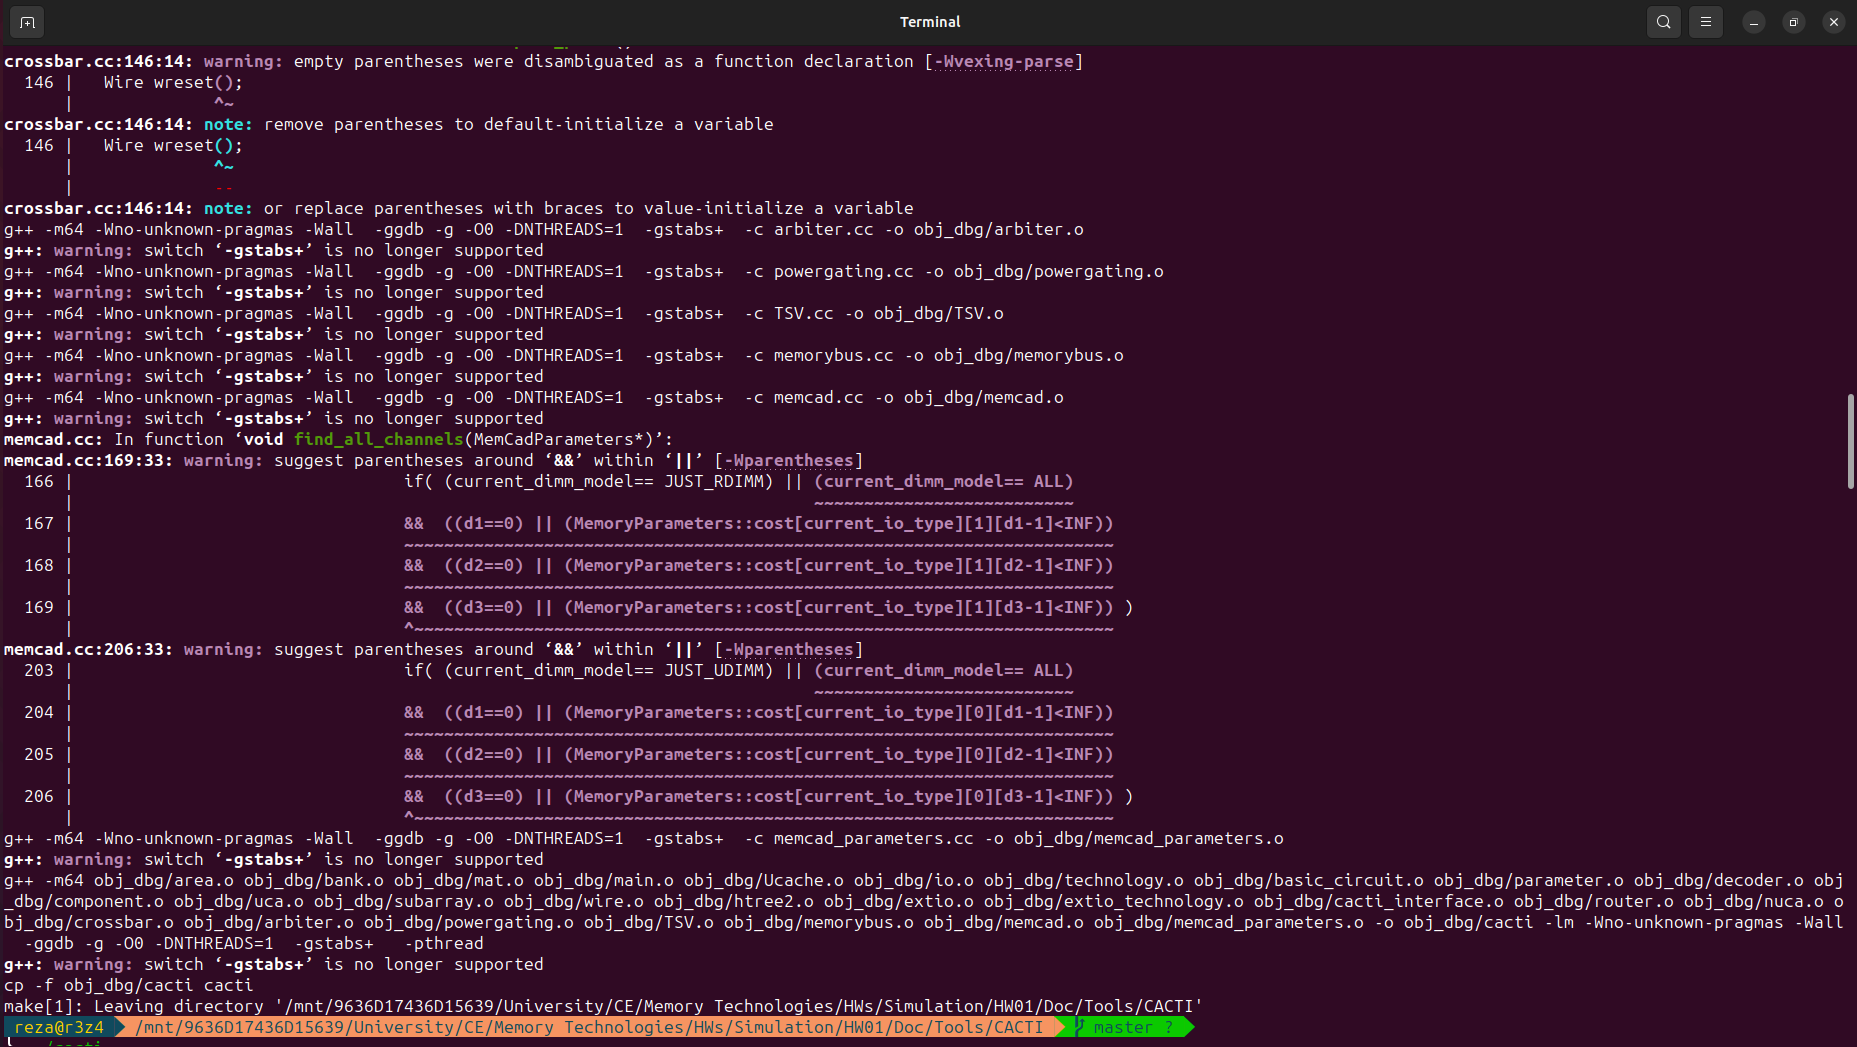
\includegraphics[height=3.5cm]{images/img3}
			\caption{Successful build}
		\label{fig:Successful build}
	\end{figure}
	
	
	%    \lstinputlisting[language=Python, label=samplecode, caption=Example of code, % firstline=1, lastline=10
	%    ]{code.py}
\end{frame}


\begin{frame}{CACTI (Cont.)}
	
	You can set cache configs in \texttt{cache.cfg} file like figure 

	
	\begin{figure}
		\centering
		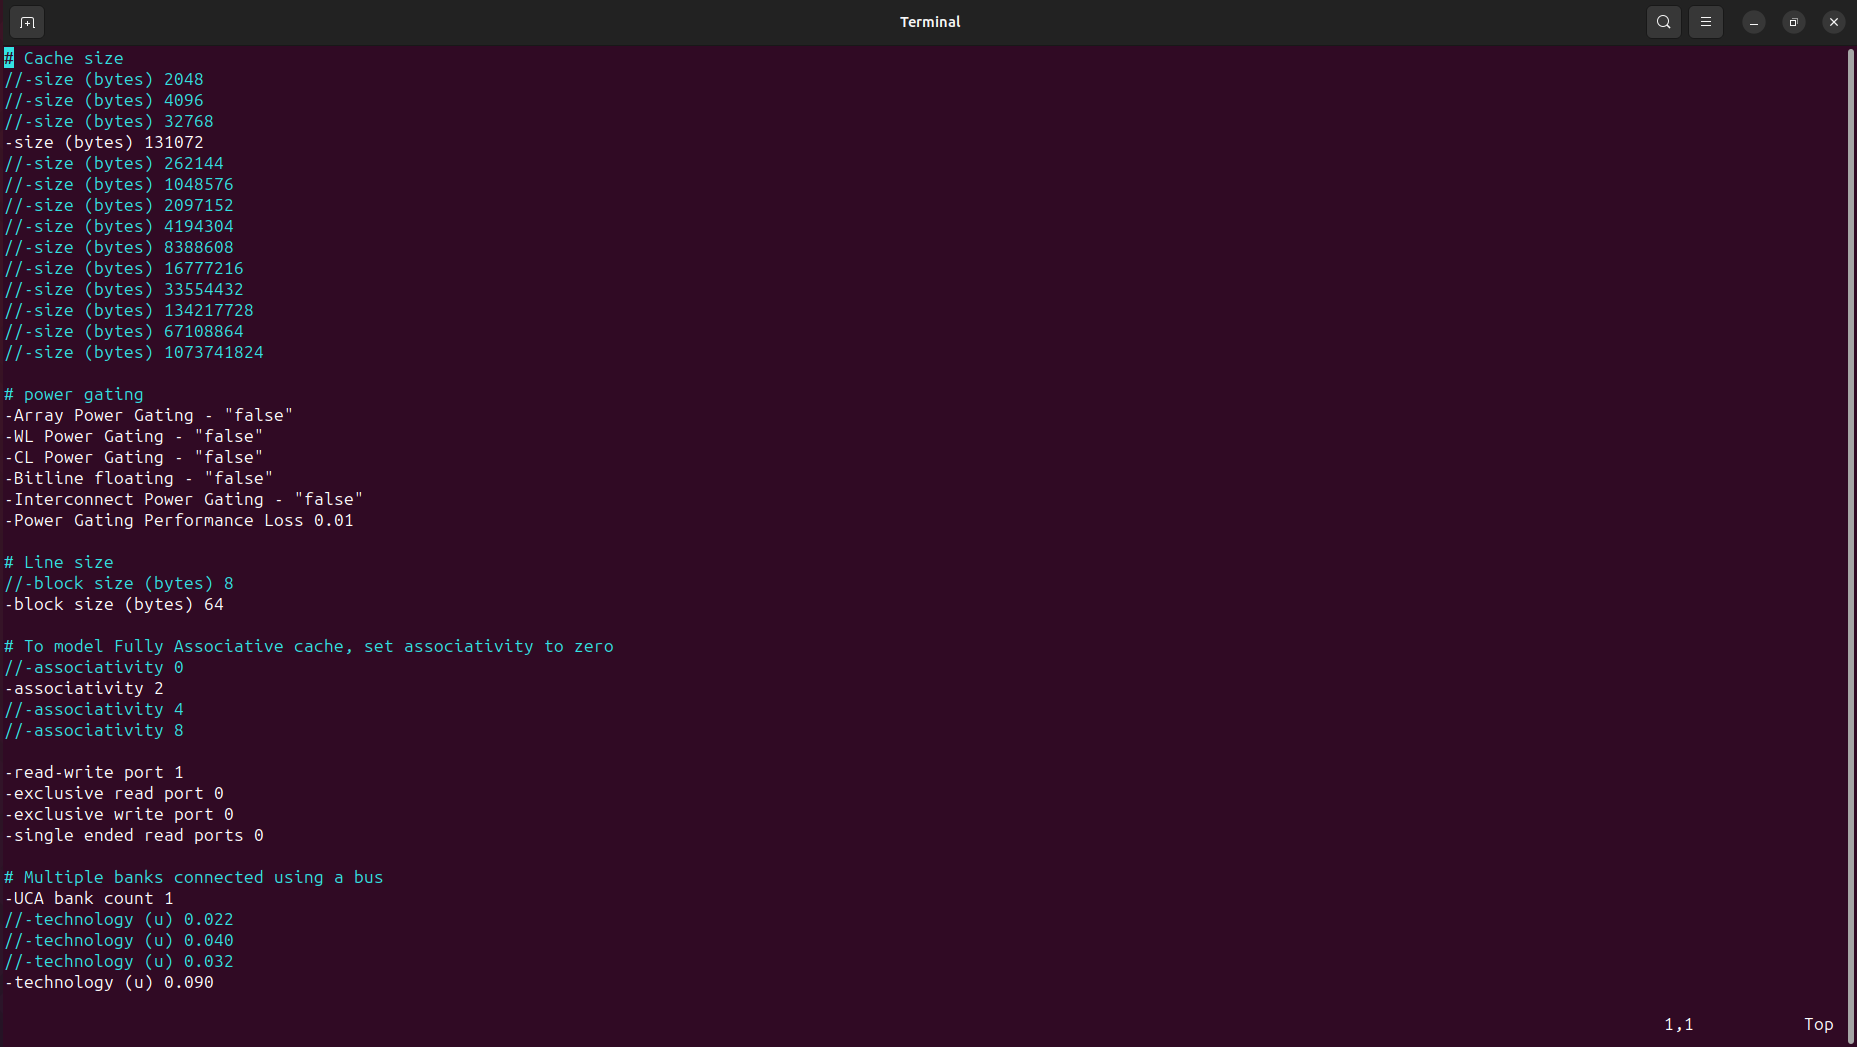
\includegraphics[height=6cm]{images/img4}
		\caption{cache config file}
		\label{fig:cache config file}
	\end{figure}
	
\end{frame}


\begin{frame}{CACTI (Cont.)}
	
	Run simulation with this command:
	
	\begin{block}{ًRun}
		\texttt{\textcolor{blue}{\$} ./cacti -infile cache.cfg}\\
	\end{block}
	
	The simulation output is as follows:
	
	\begin{figure}
		\centering
		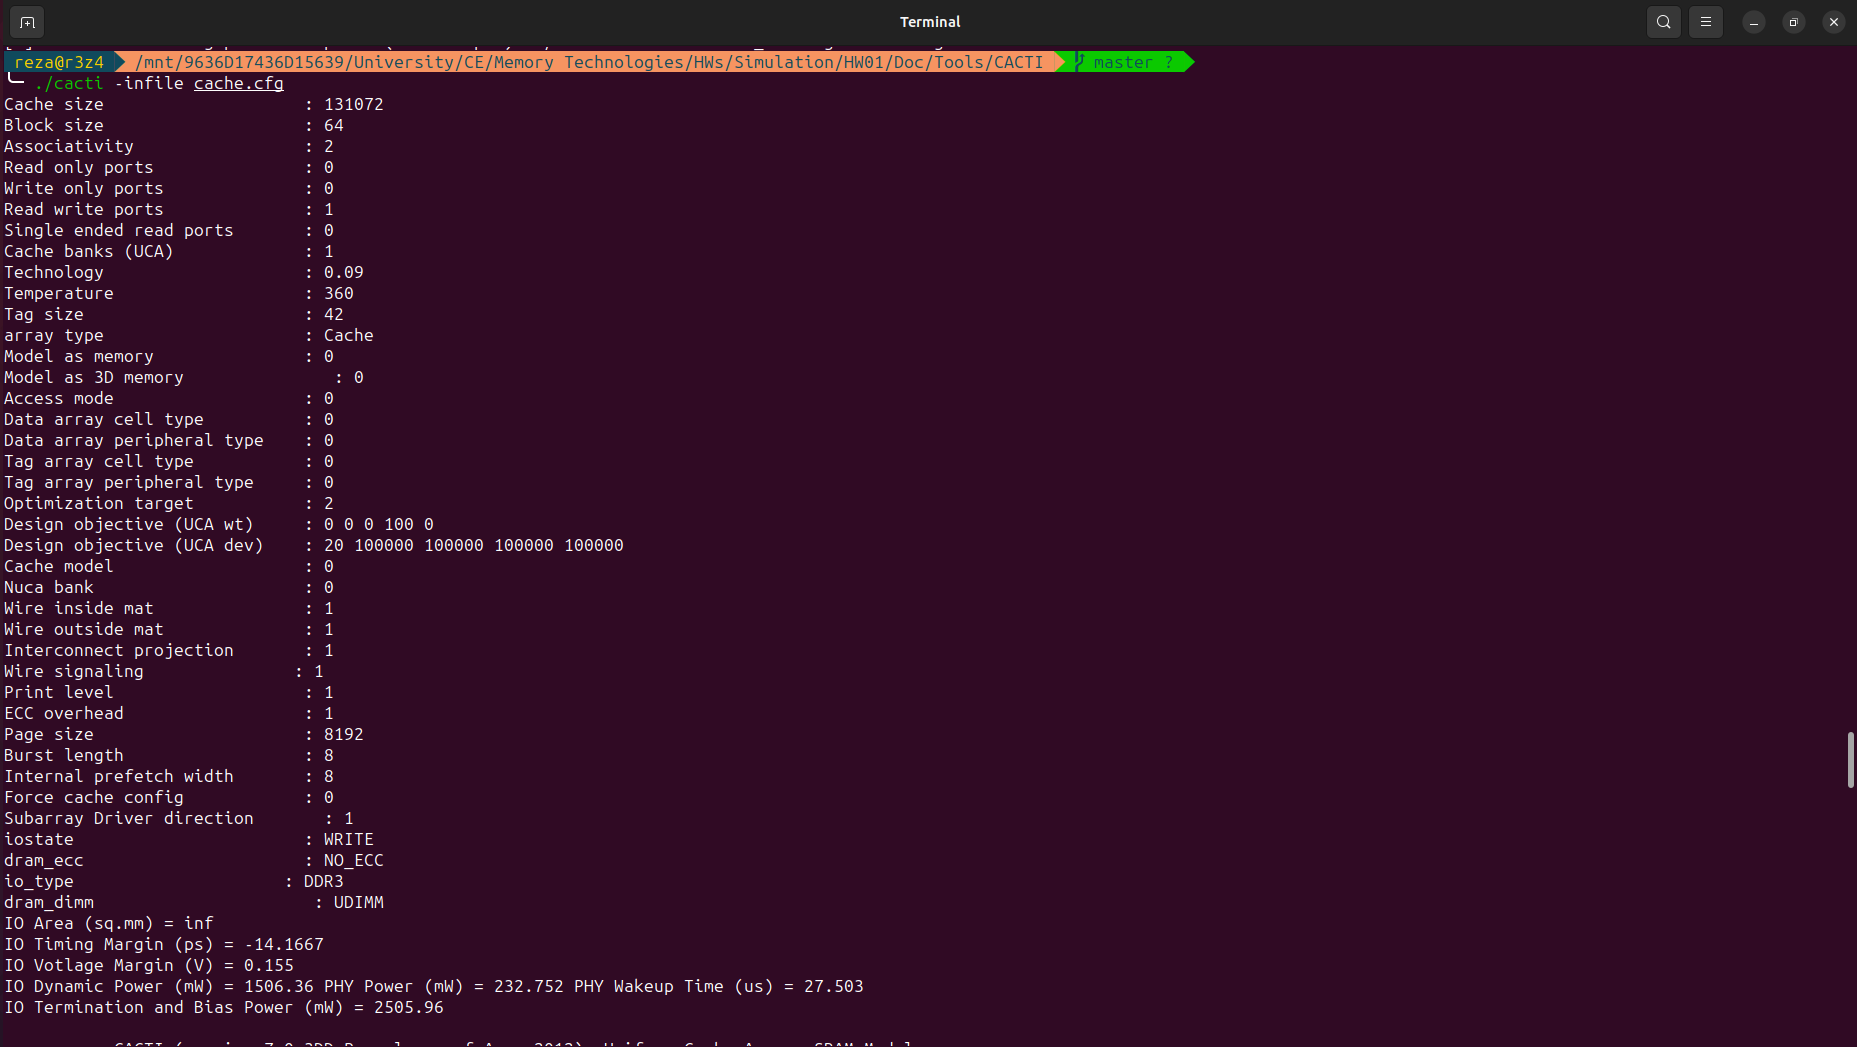
\includegraphics[height=4cm]{images/img5}
		\caption{Output report}
		\label{fig:Output report}
	\end{figure}
	
\end{frame}







%\begin{frame}{Table frame example}
%
%\begin{table}
%    \begin{tabular}{c|cc}
%        \textbf{Col1} & Col2 & Col3 \\
%        \hline
%        1            & ...                    & ...             \\
%        2            & ...                    & ...             \\
%        3            & ...                    & ...             \\
%    \end{tabular}
%    \caption{Table name}
%    \label{tab:table1}
%\end{table}
%
%\end{frame}

% --------- SECTION 3 ------- %
\section{NVSIM}

\begin{frame}{NVSIM}
	\begin{enumerate}
		\item NVSIM simulator is a tool for analyzing and simulating non-volatile memories
		\item It is primarily used for analyzing and estimating the area, power, and energy consumed
		\item Unlike CACTI simulator, NVSIM simulator supports the simulation and analysis of new emerging memories like:
		\begin{enumerate}
			\item PCM (Phase Change Memory)
			\item STT RAM (Spin Torque Transfer RAM)	
			\item ReRAM (Resistive RAM)
			\item FBDRAM (Floating Body Dynamic RAM)
			\item eDRAM	
		\end{enumerate}
		\item Developed with C++
	\end{enumerate}
\end{frame}


\begin{frame}{NVSIM (Cont.)}
	
	\begin{figure}
		\centering
		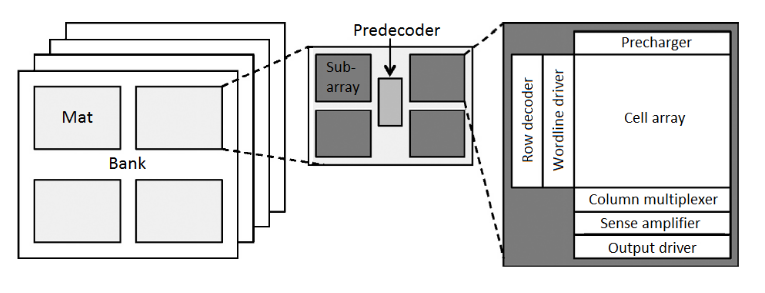
\includegraphics[height=4cm]{images/img10}
		\caption{Memory hierarchy in NVSIM}
		\label{fig:Memory hierarchy in NVSIM}
	\end{figure}

\end{frame}



\begin{frame}{NVSIM (Cont.)}
	\textcolor{green}{Advantages:}
	\begin{enumerate}
		\item Open source
		\item Support for the simulation of emerging memories
		\item low level Changeability and personalization
	\end{enumerate}
	
	\textcolor{red}{Disadvantages:}
	\begin{enumerate}
		\item Not real time
		\item There is no official version (In this talk i use modified version of simulator)
	\end{enumerate}
\end{frame}



\begin{frame}{NVSIM (Cont.)}
	\textbf{How install and compile CACTI?}\\
	
	In first clone repository: 
	\begin{block}{clone repository}
		\texttt{\textcolor{blue}{\$} git clone https://github.com/lpentecost/nvsim-merged} \\
	\end{block}
	go to repository directory and make it: 
	\begin{block}{build}
		\texttt{\textcolor{blue}{\$} cd nvsim-merged} \\
			\texttt{\textcolor{blue}{\$} make} \\
	\end{block}
\end{frame}



\begin{frame}{NVSIM (Cont.)}
	If the build is successful, your terminal output will look like this:
	
	\begin{figure}
		\centering
		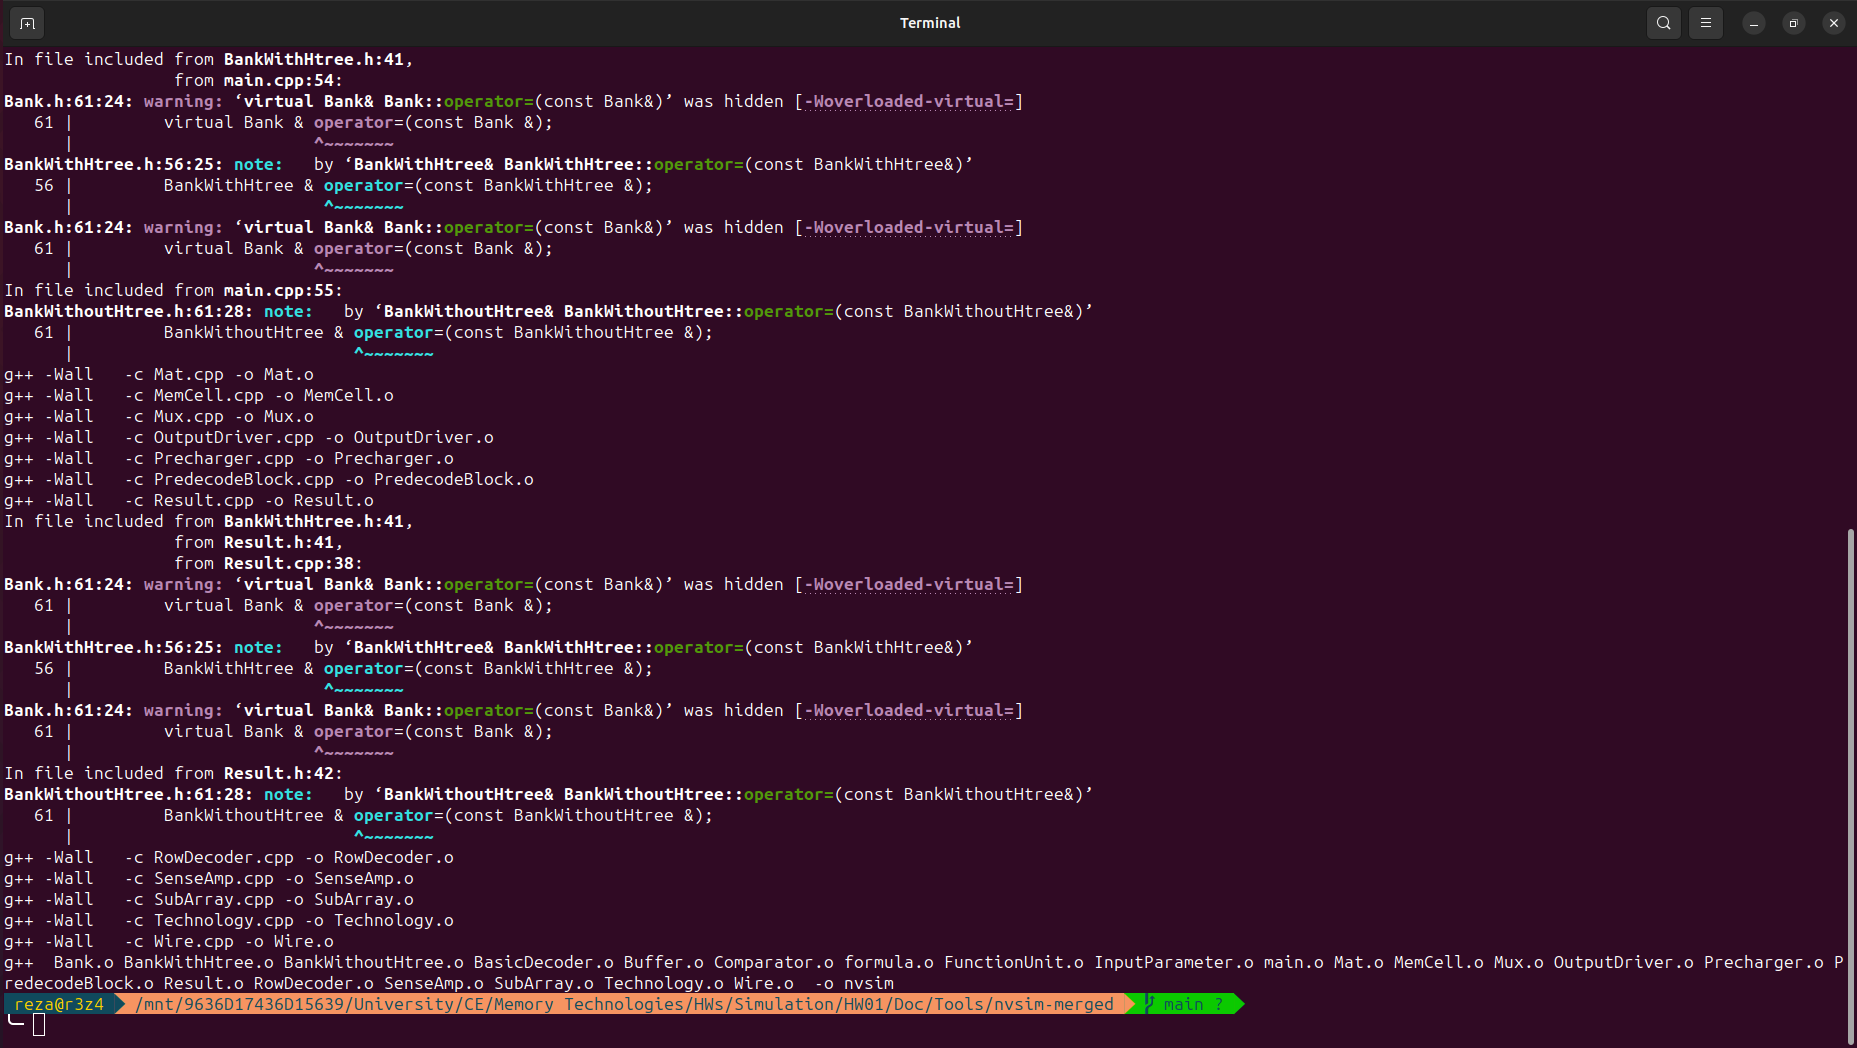
\includegraphics[height=5cm]{images/img6}
		\caption{NVSIM successful build}
		\label{fig:NVSIM successful build}
	\end{figure}
\end{frame}





\begin{frame}{NVSIM (Cont.)}
	Now we should set the config file like CACTI in \texttt{.cfg} file. for simulate simple design we use \texttt{samole.cfg} which the config of a 64 bit memristor.
	
	\begin{figure}
		\centering
		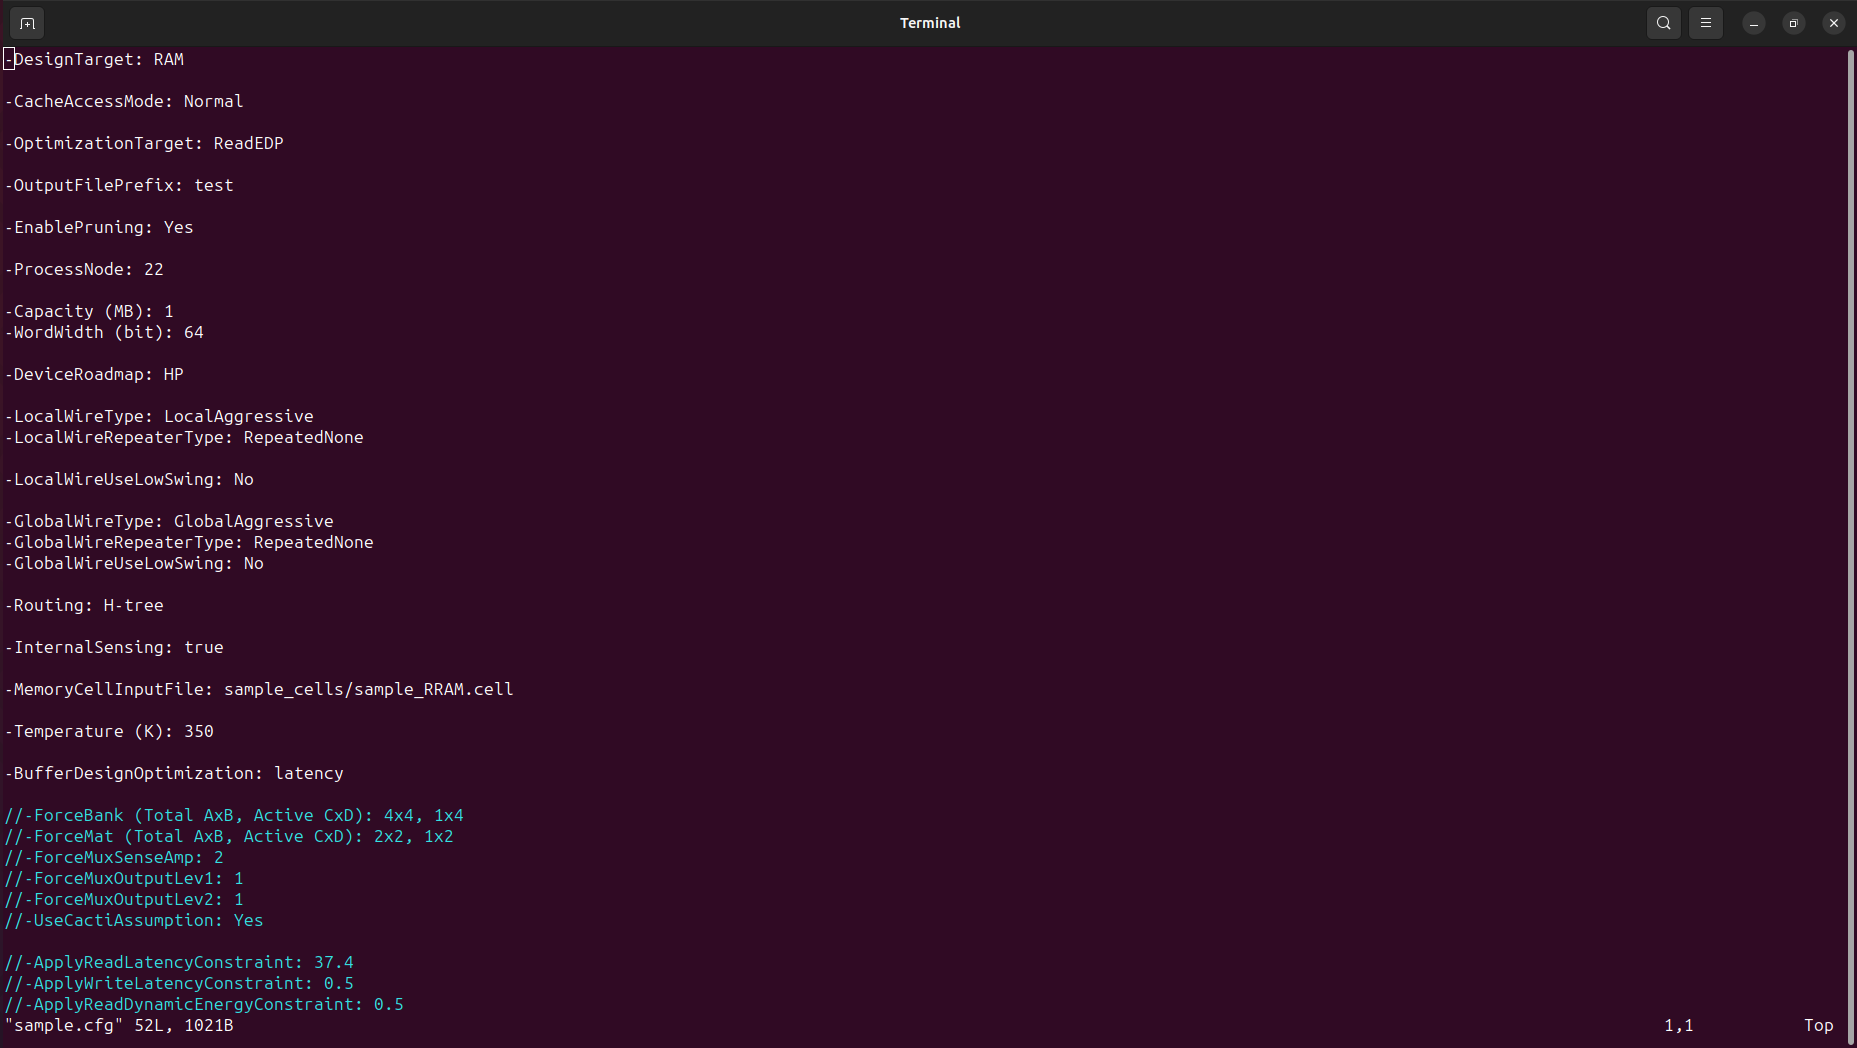
\includegraphics[height=5cm]{images/img7}
		\caption{\texttt{sample.cfg} config file}
		\label{fig:sample.cfg config file1}
	\end{figure}
\end{frame}



\begin{frame}{NVSIM (Cont.)}
	\textbf{Run simulation: }
	
	\begin{block}{Run}
		\texttt{\textcolor{blue}{\$} ./nvsim sample.cfg} \\
	\end{block}
	
	output as follow:
	
	\begin{figure}
		\centering
		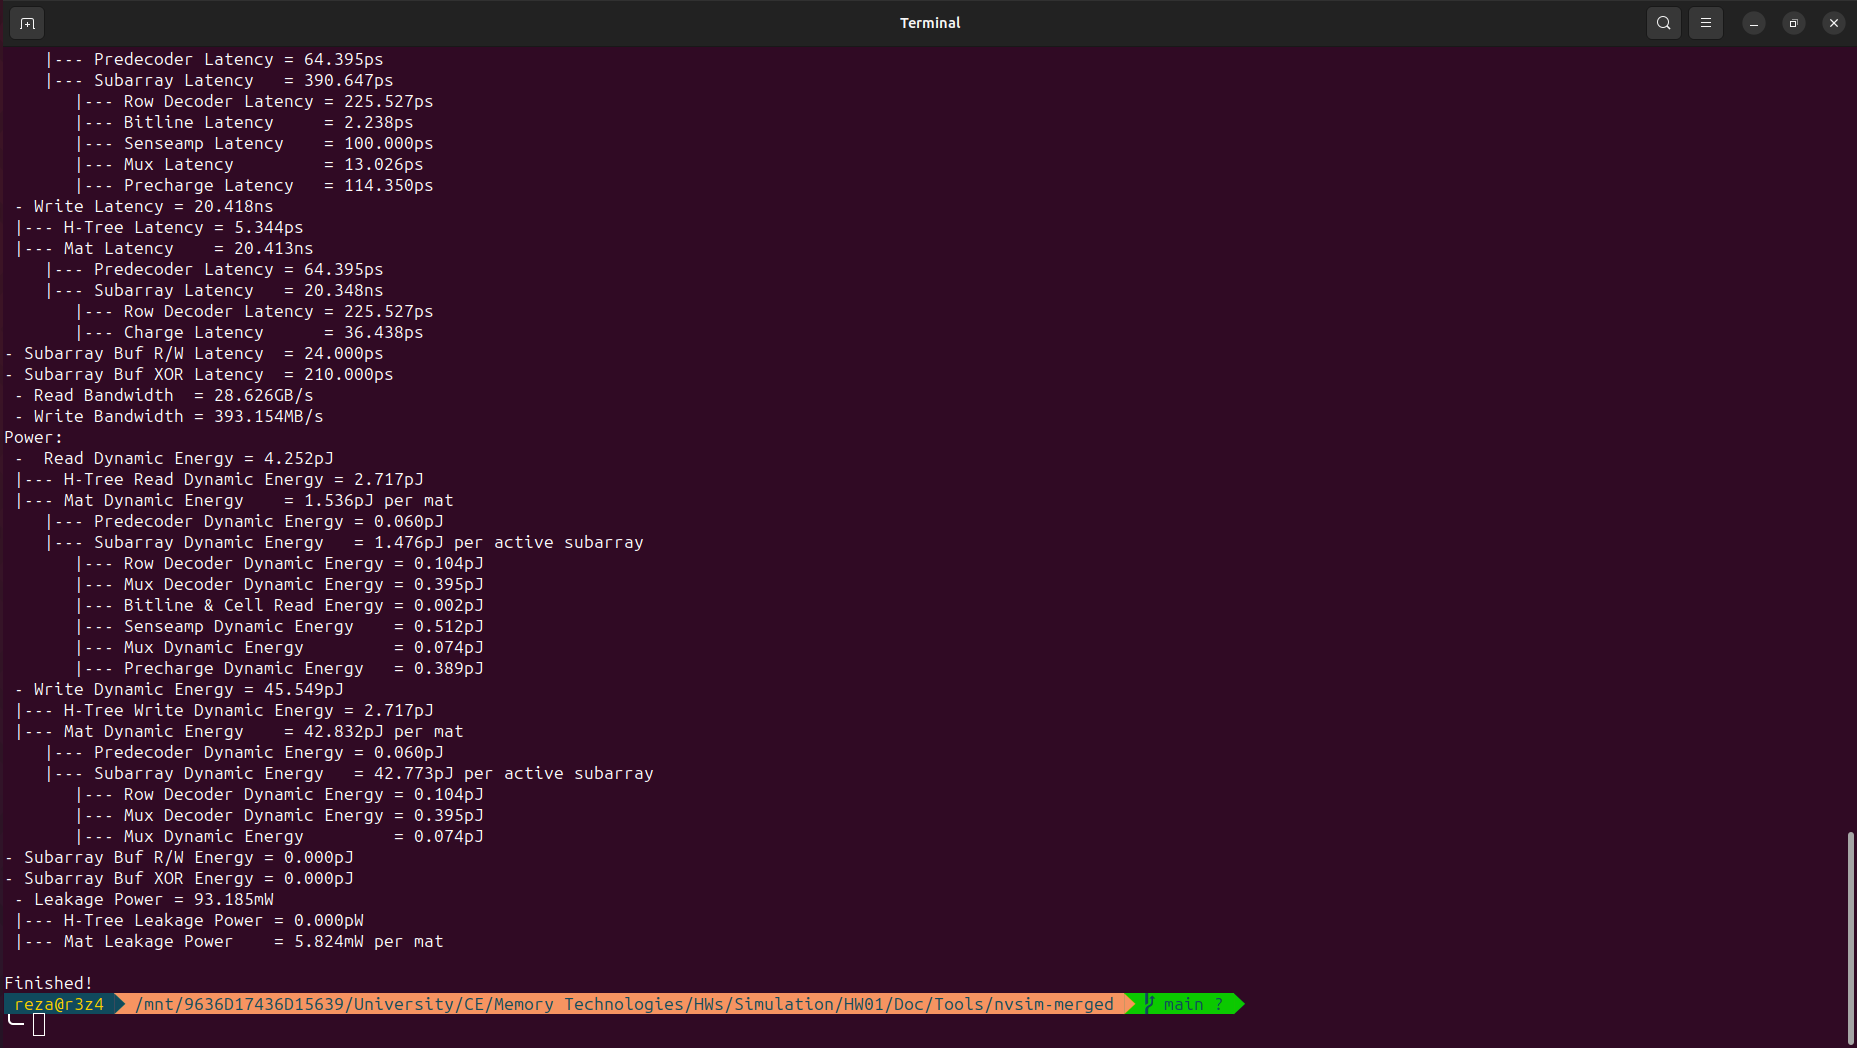
\includegraphics[height=4cm]{images/img8}
		\caption{Output of simulation}
		\label{fig:Output of simulation}
	\end{figure}
	
\end{frame}






%
%
%
%
%
%
%
%
%
%
%
%
% --------- SECTION 4 ------- %
\section{References}

\begin{frame}{References}

\hyperlink{start}{\beamerreturnbutton{Back to start}}

\nocite{bibitem1}
\nocite{*}
\bibliographystyle{IEEEtran} 
\bibliography{ref}

\end{frame}






\begin{frame}[plain]
	\begin{center}
		{\Huge To be continued}
		
		\bigskip\bigskip % Vertical whitespace
		
		{\LARGE Questions? Comments?}\\
		You can find this slides here:\\
		\textcolor{red}{\href{https://github.com/M-Sc-AUT/M.Sc-Computer-Architecture/tree/main/Memory Technologies}{\texttt{github.com/M-Sc-AUT/M.Sc-Computer-Architecture/Memory Technologies}}}
	\end{center}
\end{frame}




\end{document}
